\documentclass[12pt]{article}
\usepackage[utf8]{inputenc}
\usepackage{booktabs}
\usepackage{multicol}
\usepackage{graphicx}
\usepackage{fancyhdr}
\usepackage{lipsum}
\usepackage[backend=biber,style=verbose]{biblatex}
\addbibresource{bibliography/bibliography.bib}
\setlength{\columnsep}{4cm} % aggiusta in base alla lunghezza del tuo nome

%% ------------------------------------------------------------------- Inizio --
\begin{document}
\pagenumbering{gobble}

%% Copertina
%!TEX encoding = UTF-8 Unicode
%!TEX root = thesisCASes.tex

\begin{center}

\includegraphics[width=12cm]{figures/logo-CSC-pdf-cropped.pdf} \\
\vspace{1cm}

%{\LARGE \textbf{Conservatorio di Musica Santa Cecilia}} \\
%\vspace{0.2cm}
{\Large {Dipartimento di Nuove Tecnologie e Linguaggi
Musicali}} \\ 
%\vspace{1cm}


%{\Large {Tesi di Laurea Biennale in Musica Elettronica}} \\
{\Large {Biennio Superiore di II Livello in Musica Elettronica}} \\[2.5cm]

{\Large {Tesi di Laurea}} \\[0.5cm]

{\LARGE \textbf{Sistemi Complessi Adattivi per la performance musicale in Live Electronics}} \\[2cm]

\end{center}

\begin{multicols}{2}
\noindent \large{Relatore:} \\
\large{\textbf{Giuseppe Silvi}} \\
\vspace{0.1cm}

\noindent {\large {Correlatori:}} \\
\large{\textbf{Agostino Di Scipio}} \\
\large{\textbf{Dario Sanfilippo}} \\
\vspace{0.1cm}

%% \noindent {\large {Controrelatore:}} \\
%% \large{\textbf{Prof. Name}} \\
%% \vspace{0.1cm}
\columnbreak

\noindent{\large {Candidato:}} \\
\large{\textbf{Luca Spanedda}} \\
\end{multicols}

\vfill

\begin{center}
    \large{\textbf{Anno Accademico 2021/2022}}
\end{center}
\newpage
\
\newpage

%% ----------------------------------------------- Dichiarazione di intenti ----
\vfill
\LARGE \textbf{Dichiarazione} \normalsize \newline \newline
Dichiaro che il sottoscritto nonché autore del
documento è il responsabile del suo contenuto,
e per le parti tratte da altri lavori,
queste vengono espressamente dichiarate
citando le fonti. \\  \\
\
\hspace*{\fill} \large Luca Spanedda \normalsize
\
\newpage

%% Ringraziamenti
\vfill
\LARGE \textbf{Ringraziamenti} \normalsize \newline \newline
Prima di entrare nel merito, voglio ringraziare qui le persone
che hanno reso possibile e significativo questo percorso che ho intrapreso.
La mia famiglia, che mi ha sempre supportato durante il mio percorso.
Tutti i miei amici, che sono artisti, pensatori, e persone dal grande valore umano.
I miei compagni di corso, che sono fantastici compositori dalle idee più stravaganti,
e questi ultimi insieme ad i miei amici si sono rivelati esser
stati per me importanti compagni di vita.
Giuseppe Silvi, che mi ha accompagnato e guidato in questi ultimi anni sia da maestro
che da amico, sempre amorevolmente nel mio percorso compositivo,
ed insieme a lui, voglio ringraziare tutti i grandi Maestri e Professori
del dipartimento di Musica Elettronica,
a cui devo tanto del mio percorso, della mia crescita e del mio operato:
Pasquale Citera, Nicola Bernardini, Marco Giordano, Luigi Pizzaleo, Federico Scalas.
E il caro ex-Maestro Michelangelo Lupone, che ha formato il mio pensiero compositivo,
e che mi ha sempre incoraggiato a fare del mio meglio e rinnovare il mio entusiasmo
per la musica giorno per giorno.
E infine ringrazio di cuore Agostino Di Scipio e Dario Sanfilippo,
che sono per me grandi mentori e persone straordinarie,
e che mi hanno accompagnato in questo ultimo periodo del mio percorso,
aiutandomi e incentivandomi a portare avanti le
mie idee idee visionarie per la composizione elettroacustica,
rinnovando le mie prospettive.
Sono grato a tutti voi senza il quale questo percorso non sarebbe stato lo stesso
e non sarei giunto a questo grande traguardo,
o meglio, punto di partenza per nuovi orizzonti.
Grazie a tutti di cuore.
\newpage
\
\newpage

%% Abstract
\begin{abstract}
Il lavoro qui presentato è uno studio di analisi, implementazione e esecuzione
di tre Sistemi Complessi Adattivi per la performance musicale in Live Electronics.
La scelta di questi tre sistemi corrisponde a tre diversi casi di studio
nell'implementazione di dinamiche nonlineari sfruttate
per la generazione dei comportamenti emergenti nei Sisitemi Complessi.
Una prima parte del lavoro tratterà dell'implementazione
e l'analisi di due brani rispettivamente di Agostino Di Scipio e Dario Sanfilippo.
Di Agostino di Scipio un sistema con nonlinearità provenenti dal mondo fisico,
che sfrutta fenomeni generati dalla catena elettroacustica all'interno dell'ambiente
e riportati poi all'interno del sistema digitale.
Di Dario Sanfilippo invece un sistema che sfrutta nonlinearità
appositamente programmate dal compositore
nel mondo digitale, controllate tramite agenti di autoregolazione scritti nel software.
Infine l'ultima parte del lavoro è dedicata alla composizione di un mio brano,
che sfrutta elementi di logica ibridi appresi dai due casi di studio presentati qui,
e che andrà a conclusione del lavoro di ricerca svolto durante il corso della tesi.
\end{abstract}
\newpage
\

% conteggio pagine
\pagenumbering{arabic}

\tableofcontents
\listoftables
\listoffigures
\newpage

\pagestyle{fancy}

%% --------------------------------------------------- Capitoli ----------------
%% capitolo TEST
%%\input{chapters/0_TEST}
%% TITOLO
\section{Introduzione}
\label{sec:Introduzione}

%% TESTO
Dopo la crisi del sistema tonale (in uso in Occidente dal XVII secolo)
e dopo la crisi dei fondamenti delle scienze di inizio secolo,
le nascenti considerazioni strutturali e teoriche
nella musica alla ricerca di vie al di fuori del sistema tonale,
parallelamente all'esigenza di introdurre nuovi paradigmi all'interno delle scienze,
hanno contribuito all'avvenire di importanti punti di incontro fra i due ambiti.
\\
Uno dei più importanti avanzamenti nelle scienze
al termine della seconda guerra mondiale, risedette nell'introduzione della
cibernetica e della teoria generale dei sistemi, che hanno conseguentemente
portato alla nascita del pensiero sistemico e del concetto di scienze della complessità.
\\
La cibernetica in particolare ebbe inizio durante gli anni della seconda guerra mondiale e si deve al fisico e matematico Norbert Weiner.
Nel 1940 Wiener insieme ad altre ad altre prominenti figure provenienti da diversi ambiti scientifici,
come Ross Ashby, Margaret Mead, Gregory Bateson, Heinz von Foerster, partecipano ad una serie di conferenze
multidisciplinari chiamate "The Macy Conferences", inizialmente intitolate
"Feedback Mechanism in Biology and the Social Sciences" con l'obiettivo comune di andare a definire
gli ambiti di interesse della nuova scienza.
Il concetto sviluppato dai greci - kybernetes -
viene poi ripreso da Norbert Weiner nel 1948,
che ispirato dalla meccanica ed i suoi risultati durante la guerra
e contemporaneamente dallo sviluppo della teoria della comunicazione (o informazione) di Claude Shannon,
con la volontà di sviluppare una teoria generalizzata dei principi di
organizzazione e controllo nei sistemi emersi durante le conferenze pubblicherà un libro nel 1948:
La cibernetica, controllo e comunicazione nell'animale e nella macchina,
in cui definiva l'ambito di interesse e gli obiettivi della nuova disciplina,
inaugurando anche l'uso del nuovo termine da lui coniato; a seguito di questo libro che riscuoterà
un importante successo, le conferenze presero il nome di
"Cybernetics, Circular Causal, and Feedback Mechanism in Biological and Social Systems",
innalzando Wiener come la principale figura di spicco.
\\
La cibernetica è la scienza che studia i principi astratti di organizzazione
nei sistemi complessi.
In particolare come evidenziato fino ad ora dalla sua natura multidisciplinare,
non si interessa con particolare attenzione in cosa consistano questi sistemi,
quanto al più al loro funzionamento:
\\
- come usano l'informazione e come la scambiano gli agenti
\\
- come collaborano fra loro in direzione di un obiettivo comune
\\
- come contrastano il rumore
\\
e così via...
\\
Le fortunate premesse iniziali della cibernetica risiedevano in una convinzione
da parte di questi scienziati provenienti dai differenti ambiti disciplinari, che esistesse uno
"schema processuale" comune ad organismi viventi e macchine, rintracciato attraverso una ricerca uniforme garantita da dell'utilizzo di un metodo "sintetico" e "comportamentale".
Fra gli anni '60 e la metà del '70 la cibernetica grazie agli scienziati
Heinz von Foerster, Margaret Mead, e altri,
compierà un ulteriore passo fondamentale che la porterà
verso il compimento della stessa in una scienza concreta, divenendo la "Cibernetica di secondo ordine",
anche chiamata come "la cibernetica dei sistemi di osservazione", che consiste nell'applicazione
ricorsiva della cibernetica a se stessa e la pratica riflessiva della cibernetica
secondo tale critica.
La differenza fra cibernetica di primo e secondo ordine risiese nel fatto,
che mentre nel primo periodo lo studioso di cibernetica (di primo ordine)
studiava un sistema da un punto di vista passivo, da quello dell'osservatore
dei comportamenti di un sistema.
Il  cibernetico di secondo ordine lavora ed interviene nel comportamento
e nella costruzione di un sistema complesso,
riconoscendo il sistema come un agente con cui interagire e
riconoscendo esso stesso come agente nell'interazione col sistema.
\\
A partire dalle sue importanti premesse,
la cibernetica ha conseguentemente poi avuto un ruolo centrale nello sviluppo di
molti studi scientifici e la nascita
di nuovi ambiti come: l'intelligenza artificiale, la teoria del caos,
la teoria della catastrofe,
la teoria dei controlli, la teoria generale dei sistemi, la robotica,
la psicologia e le scienze sociali,
ecc.
nella mappa di B.Castellani e L.Gerrits riportata per intero nella pagina seguente,
possiamo visualizzare con più precisione e accurtezza
l'insorgere e l'evoluzione di questi paradigmi scientifici, per averne una
visione più completa relativa al loro sviluppo.

\clearpage

\begin{figure}[!h]
    \centering
    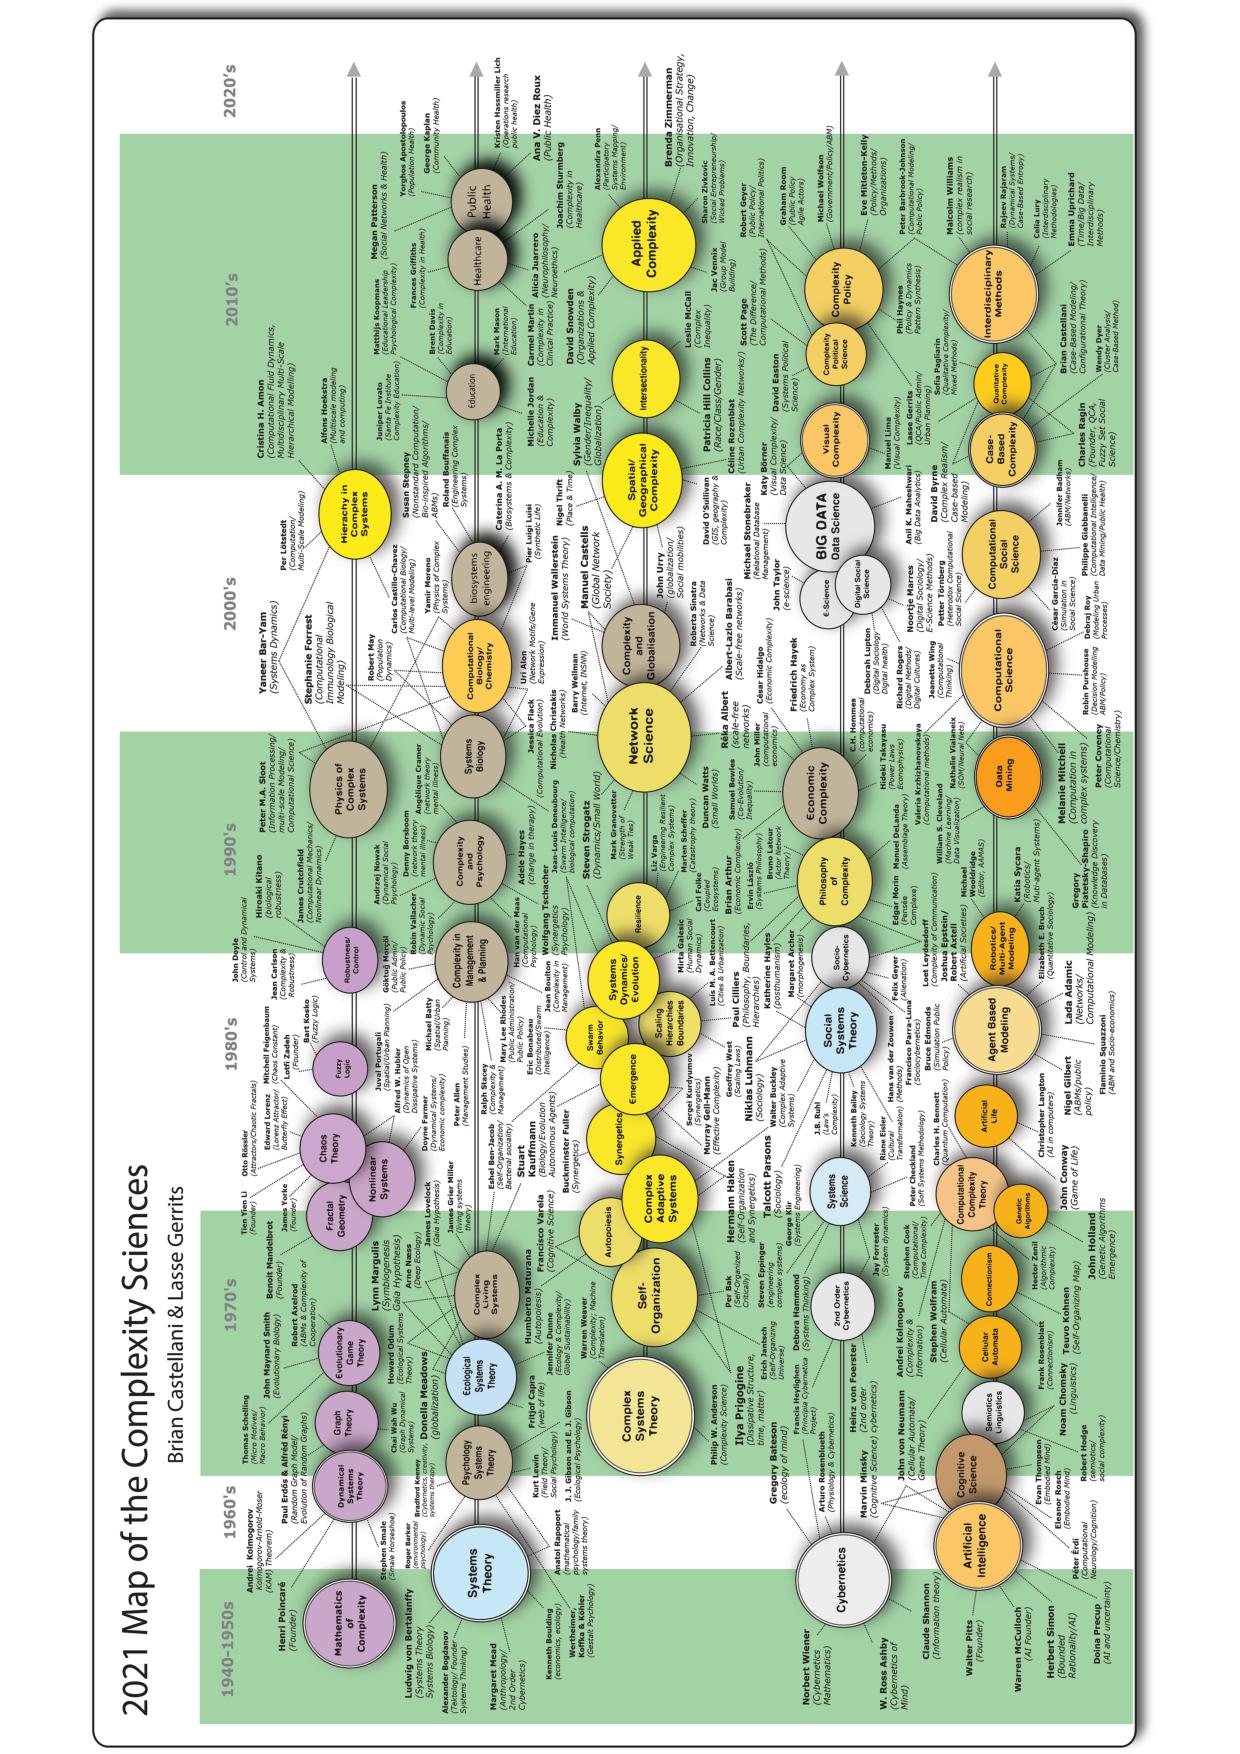
\includegraphics[width=1.0\textwidth, angle=0]{figures/complexitymap.pdf}
    \label{fig:figure}
\end{figure}
%% https://www.art-sciencefactory.com/MapLegend.html

\clearpage

\subsection{Le cibernetiche nella musica}
\label{sec:Le cibernetiche nella musica}
All'inizio degli anni '60 in seno alle nascita delle scienze complesse,
l'uso di sistemi di feedback e la rilevanza dei circuiti informativi chiusi
nelle strutture organizzate,
ha goduto di uno slancio popolare anche nel mondo della musica e più in generale dell'arte.
Uno dei primi nella storia dell'arte ad evocare l'uso della cibernetica nei propri lavori è stato
Nicolas Schoeffer con il suo ciclo di lavori "spazio-dinamici", in particolare ha creato
la prima installazione ad implementare meccanismi di auto-regolazione, il CYSP-1,
capace di essere sensibile all'ambiente esterno e a se stesso
grazie ad una serie di tecnologie offerte dalla compagnia Philips (fotocellule e microfoni),
e reagire sonoramente a questi stimoli riproducendo
una serie di registrazioni composte dal compositore francese Pierre Henry,
collaboratore di Pierre Schaeffer ed insieme a lui figura centrale nella nascita della Musique concrète.
Un'altra importante esperienza del periodo iniziale è quella del compositore Roland Kayn,
che dopo essersi avvicinato alla musica elettronica sotto la guida di Herbert Eimert
nello studio di Colonia (1954),
e dopo essersi trasferito a Roma nel 1960, dal 1964 assieme ad Aldo Clementi e Franco Evangelisti
fonda il Gruppo di improvvisazione Nuova Consonanza, del quale fece parte sino al 1968,
ed in quel periodo ispirato dalle teorie della cibernetica iniziò a sperimentare
estensivamente con sistemi di autoregolazione basati su feedback loops,
sia come modelli formali per composizioni strumentali che come reti di generatori di segnale analogici.
Tuttavia, a parte casi popolari di deliberate dichiarazioni formali da parte degli artisti,
come è nel caso di Roland Kayn,
non bisogna pensare a questi lavori appena citati (ed altri riportati a seguito),
come ad atti pioneristici che sancisono la nascita della cibernetica in musica,
ma proprio come si dice per la scoperta del fuoco
lo scenario più accurato risiede probabilmente nel fatto che
tanti autori provenienti da diverse parti del mondo, nello stesso periodo
sono stati influenzati e si sono influenzati a vicenda con le stesse idee
provenienti da un interesse condiviso per le teorie cibernetiche di Weiner e delle Macy Conferences.
Si può pensare ad esempio a quelle che sono le esperienze dello studio di Colonia:
nel 1951, Herbert Eimert e Werner Meyer-Eppler persuasero il direttore della NWDR, Hanns Hartmann,
a creare uno Studio per la Musica Elettronica, che Eimert diresse fino al 1962.
Questo è diventato lo studio più influente al mondo durante gli anni 1950 e 1960,
con ospiti alcuni dei più importanti compositori contemporanei provenienti da tutta europa,
come il già citato Roland Kayn, Franco Evangelisti, Karlheinz Stockhausen, Herbert Brun,
Cornelius Cardew, e molti altri.
Qui è dove nel 1964 K.Stockhausen lavora a "Mikrophonie I", che seppure non dichiarato è un ovvio punto di inizio
se si pensa a quelle logiche di interazione sistemiche fra uomo/macchina/ambiente in musica,
e in quel caso un punto di formalizzazione importante per quella che sarà l'esperienza del live electronics,
e non a caso in quel periodo il lavoro di ricerca condotto da Werner-Meyer Eppler,
scienziato, musicista ideatore e direttore dello studio di Colonia,
ha trovato sin dalla nascita dello studio fondamento in quelle che sono state
le teorizzazioni della Cibernetica.
Parlando sempre dello studio di colonia, c'è poi il caso di Franco Evangelisti,
come citato prima fondatore insieme a Roland Kayn del Gruppo Improvvisazione Nuova Consonanza,
che in quel periodo (qualche anno prima della fondazione del Gruppo a Roma)
si trova nello studio di Colonia per lavorare al brano "Incontri di Fasce Sonore",
e quando farà ritorno a Roma poi citerà più volte deliberatamente in interviste, scritti,
e altre documentazioni, il suo approccio sistemico/cibernetico a quelle che saranno le esperienze con
Gruppo.
O ancora, se cambiamo paese e passiamo dall'Europa od osservare l'America in quel periodo,
possiamo pensare a quelli che sono i lavori di Louis e Bebe Barron,
con i circuiti in retroazione destinati al corto circuito
e utilizzati appositamente come materiale per la generazione acustica di trame incise su nastro,
o ai lavori di John Cage come "Electronic Music for piano" o di Steve Reich come "Pendulum Music" del 1968,
che sfruttano ed esplorano l'effetto Larsen in modo artistico.
\\
Un secondo periodo costituito da un approccio sistemico più consapevole
che inizia a tracciare la strada per un pensiero ecosistemico della composizione, inizia dal lavoro
di Alvin Lucier, che nel 1969 scriverà quello che sarà un brano emblematico per
la cibernetica in musica "I'm sitting in a room", altro brano importante per quelle che sono
le logiche di interazione sistemiche fra uomo/macchina/ambiente e che sancisce una volta per tutte
l'interazione sistemica dove il musicista l'ambiente e lo strumento sono parti di un insieme del
sistema "più complesso" con un comportamento collettivo derivato dai singoli agenti,
in un un'interazione con l'ambiente circostante.
In I'm sitting in a room, un performer al centro della stanza
recita in un microfono un testo che descrive il fenomeno che avverrà poco a poco,
la voce recitante nel microfono viene registrata e poi riprodotta da altoparlanti
posti nella stanza, il suono della regitrazione riprodotta da questi altoparlanti
viene registrato nuovamente durante la riproduzione, l'operazione
viene ripetuta in un in una casualità circolare di volta in volta dove alla fine rimarranno
solo i contributi provenienti dalla stanza, dalla voce e dalla catena elettroacustica,
dando vita nel loro insieme ad un effetto Larsen, la natura
nonlineare del processo e degli agenti porterà di volta in volta ad un risutato
sempre differente.
Dopo l'esperienza di Lucier, nel 1974 Nicolas Collins compone "pea soup"
mentre è studente alla Wesleyan University.
Pea soup consiste in una rete adattiva di circuiti analogici (3 Countryman Phase Shifters),
che intona il feedback positivo dell'effetto Larsen ad una frequenza risonante diversa
ogni volta che questo inzia ad emergere.
Ad oggi svariati compositori a partire dalle trame delineate dalle scienze complesse e
dai lavori citati operano nell'ambito della musica elettronica con un approccio sistemico,
un importante caso è quello di Agostino Di Scipio, che contribuisce significatamente
nell'ambito della computer music sin dai primi anni '90, divenendo una
delle figure più importanti nell'area della composizione ecosistemica e nel suo
caso in particolare del live electronics, o quello di Dario Sanfilippo
compositore e ricercatore con all'attivo recenti importanti pubblicazioni e lavori
nell'ambito dei sistemi di feedback in musica, e in particolare di non linearità nei sistemi
in DSP.

\clearpage
%% TITOLO
\section{La composizione di interazioni ecosistemiche}
\label{sec:La composizione di interazioni ecosistemiche}

%% TESTO
Si parla spesso di “interattività”. la storia delle “arti interattive” è documentata da una gran mole pubblicazioni, tra le
quali molte naturalmente si occupano di “musica interattiva”.
1

\clearpage
%% TITOLO
\section{Sistemi Autonomi}
\label{sec:Sistemi Autonomi}

Nel capitolo precedente, attraverso la composizione e gli studi di Agostino Di Scipio, 
abbiamo potuto osservare che cosa si intende, e come viene organizzato, 
un sistema con non linearità provenienti dal mondo fisico; aperto al suo ambiente esterno 
che diviene in questo caso lo spazio stesso della performance.
Sempre in riferimento alla cibernetica di secondo ordine,
abbiamo già parlato del fatto che nessun sistema è separabile e 
isolabile da un suo ambiente circostante, 
ma abbiamo osservato anche come il concetto di spazio di un sistema sia 
qualcosa di molto complesso, poiché il concetto stesso di "complessità"
sta a significare in un sistema che questo sia composto da una rete d'interazioni dinamiche, 
ma che il comportamento dell'insieme potrebbe non essere prevedibile in base al comportamento 
dei diversi componenti tipicamente in relazione fra loro.
Mentre, nel caso di Agostino Di Scipio, lo spazio del sistema che ne contiene le sue relazioni 
è costituito principalmente dal mondo fisico, 
in questo capitolo osserveremo come, per lo spazio di un sistema, 
si possa intendere anche uno spazio latente, 
che traccia le sue relazioni tra le parti in uno spazio virtuale interamente programmato nel software. 
In questo caso, l'ambiente digitale che racchiude il sistema all'interno e le sue relazioni 
tra gli agenti è interamente costituito solo dal DSP, 
inclusi i metodi per la generazione delle relative non linearità.
Ho voluto approfondire questo metodo attraverso il lavoro compositivo e gli studi di Dario Sanfilippo, 
specialista di sistemi di feedback, esecutore e compositore. 
I suoi lavori riguardano principi di autopoiesi, evolvibilità e costruttivismo radicale nella progettazione 
di reti di feedback audio complesse. \\
La modalità con cui andrò a discutere in questo capitolo la composizione di questi
sistemi autonomi, appartenenti anche questi alla più vasta categoria dei CASes (Complex Adaptive Systems), 
è ponendo un focus su un particolare lavoro di Dario Sanfilippo, Order From Noise \textit{(Homage to Heinz Von Foerster)}. \\
Order From Noise \textit{(Homage to Heinz Von Foerster)} è un progetto che implementa uno 
dei primi prototipi di Dario Sanfilippo basati sull'idea dell'\textit{adattattività dinamica}. 
Questo lavoro del compositore si basa sull'idea che i sistemi adattivi complessi, 
che sono emergenti per definizione, siano essenziali per raggiungere innovazioni formali, 
performative e tecniche, nel contesto della performance in Live Electronics e nella composizione musicale in generale. 
\footcite{sanfilippo_time-variant_2018}
I CASes si dicono adattivi quando sono composti da una rete dinamica 
di interazioni dove i singoli agenti interconnessi fra loro, interagendo individualmente
o collettivamente, possono cambiare il loro stato in risposta a variazioni nell'ambiente o
degli altri agenti connessi. 
Questo tipo di relazioni nel sistema è comune sia nell'opera di Agostino Di Scipio,
in cui abbiamo visto precedentemente come lo stato dei singoli agenti nel sistema 
cambi al variare delle condizioni nell'ambiente circostante portando a
cambiamenti di stato globali del sistema, che nel lavoro di Dario Sanfilippo.
Altro importante aspetto in comune qui con l'opera di Agostino Di Scipio,
è il tipo di rapporto che ha l'uomo con la macchina, che viene respinto nella visione in cui è il primo
ad essere totalmente a controllo del secondo, per essere sostituito da un concetto 
d'interazione Uomo-Macchina-Ambiente, chiamato da Dario Sanfilippo Ibridazione: 
una condizione in cui umano e macchina cooperano per far emergere la performance. 
Nel caso delle opere di Dario Sanfilippo, tuttavia, l'estetica dei suoi lavori è interamente subordinata
al disegno del sistema stesso, che di volta in volta, emerge da fenomeni musicali che sono il risultato
del tipo d'interazione che viene a crearsi fra il performer e il disegno del sistema che si era reso necessario
in partenza. \\
In alcuni casi, questa idea viene portata alle sue estreme conseguenze con opere in cui la macchina è l'unica 
ente che esegue, come accade per il brano presentato qui.

\begin{center}
    \vspace{0.5cm}
    \textit{Order from noise (2017) is based on a time-variant feedback delay network containing a 
    set of entangled nonlinear processing algorithms for audio and information signals. 
    The work is an example of autonomous self-performing system and it is realised by
    feeding the network with one millisecond of background noise from the performance
    environment. The initial recirculating noise impulse is what entirely determines the
    formal evolutions of the system which have substantially different long-term developments 
    for each different noise impulse. An approach to present the work live is that
    of reinitialising the system a number of times for a period of about three-five minutes
    to show its sensitivity to initial conditions and the long-term divergence between the
    formal structures.}\footcite{sanfilippo_time-variant_2018}
    \vspace{0.5cm}
\end{center}

Rispetto al sistema discusso nel capitolo precedente, 
come già accennato c'è una sostanziale differenza nel concetto di spazio
o ambiente del sistema. 
Come appena detto, Order From Noise è basato su una \textit{feedback delay network} 
tempo-variante, vuole dire che ci ritroviamo di fronte ad un un sistema il cui
funzionamento cambia nel tempo, a differenza dei sistemi tempo-invarianti
dove seppur l'output del sistema può cambiare nel tempo, 
il loro funzionamento e l'ambiente che contiene il sistema rimane inalterato.
In parole semplici lo spazio del sistema in Order From Noise può variare nel tempo,
rendendo imprevedibile il suo funzionamento a partire da una determinata condizione 
iniziale.
Per questo motivo il performer non avrà un grande margine di prevedibilità 
nel comportamento del sistema a differenza dei sistemi tempo-varianti,
ma saprà che per le stesse condizioni iniziali, il sistema qui totalmente
deterministico, riporterà sempre le stesse evoluzioni formali.
Proprio come nei Sistemi Caotici emersi dalla Teoria del Caos introdotti all'inizio di questa tesi,
che seppur governati da leggi deterministiche, 
sono in grado di esibire un'empirica casualità nell'evoluzione delle variabili dinamiche. \\

\subsection{Audio Information Processing}
\label{sec:Audio Information Processing}
Come già accennato nello scorso capitolo, l'\textit{Audio Information Processing};
ovvero la capacità di un sistema di elaborare le informazioni
tremite la \textit{feature extraction}, è un dato fondamentale nella creazione 
di un CAS, che ne determina le sue capacità "congitive" e di auto-osservazione
rispetto all'ambiente. L'uso creativo dei CASes in Musica,
e la loro stretta connessione con l'informazione,
ha favorito lo sviluppo di techniche algoritmiche per \textit{Audio Information Processing} 
e l'analisi di comportamenti ad alto e basso livello.
Alcuni primi alcuni esempi storici sono ad esempio le performance 
in Live Electronics di Gordon Mumma, 
come ad esempio “Diastasis, as in Beer” (1966), e "Hornpipe" (1967), 
dove vengono implementate techniche di amplitude following utilizzate 
poi per pilotare parametri nelle unità di generazione del suono.\footcite{sanfilippo_time-domain_2021}


\begin{center} \vspace{0.5cm} \Huge - Da Continuare - \normalsize \vspace{0.5cm} \end{center}

Lookahead Limiters per la stabilità delle Feedback Network:
In Order From Noise Dario Sanfilippo utilizza un unità per raggiungere la stabilità
globale della rete chiamata Lookahead Limiter.
<< My original design was based on two side-chained amplitude curves: 
a fast one for attack transients and one for sustained sounds, which had 
to be slow enough as to avoid intermodulation distortion. The fast curve 
was based on peak envelope estimation (see below), while the slow one was based on 
RMS to have a smooth behaviour. The curves were in a master-slave mode so that 
the effect of the fast curve would decrease with regard to the growth of the slow curve: 
that was necessary to avoid that the processed signal would be scaled down twice by both curves. 
Despite the algorithm produced good results, it needed some empirical calibrations 
and it also involved a rather large number of objects in Pure Data which would considerably load the CPU. 
Besides, I was using some objects from PD-extended and I already had in mind to migrate to Pure Data Vanilla.
A simplified design was based on only one amplitude curve calculated with a long-decay peak envelope (10 seconds). 
A peak envelope checks whether the input is greater than the output and, if that condition is true, 
it updates the peak with the new value from the input signal. 
Otherwise, the current peak decreases following an exponential curve and reaches a certain 
attenuation after a desired time which, in my specific case, is of ~60dBs. 
This would allow detecting fast attack transient and, at the same time, 
the long decay would create a smooth curve for the sustained and slow sounds. >>
https://www.dariosanfilippo.com/blog/2017/lookahead-limiting-in-pure-data/

This was a good compromise for my systems, although such a long decay is not always desirable: occasionally, 
that would create silences after high-amplitude impulses for the attenuating curve 
would decrease very slowly and the input signal would be scaled down even if below the limiting threshold.
\clearpage
%% TITOLO
\section{RITI: un sistema caotico ibrido}
\label{sec:RITI: un sistema caotico ibrido}

RITI : Room Is The Interface è un Brano basato su un CAS autonomo \textit{site-specific},
dove la personalità acustica della stanza dove viene eseguito il brano
viene riflessa in variazioni del comportamento del sistema stesso.
L'idea dell'acronimo RITI nasce come omaggio a: Sound is the interface, 
il famoso paper di Agostino Di Scipio, che introdusse per la prima volta
una prospettiva sistemica sull'auto-organizzazione e sulla capacità
di un sistema di auto-osservarsi tramite l'ambiente circostante. \\

\subsection{Motivazioni}
\label{sec:Motivazioni}

In questi ultimi anni di studi musicali, sono emerse nel mio fare musica 
delle questioni per me di fondamentale importanza che hanno accompagnato il mio operato
e che giustificano la mia esigenza di essermi interessato ai CASes in musica. \\
In primo luogo indagare rispetto al rapporto che esiste fra l'interprete, la notazione, e lo strumento musicale;
che può essere vista come una parte contenuta all'interno della relazione fra uomo-macchina-ambiente di cui parla
Agostino Di Scipio. \\
Le prime forme di semiografia musicale possono essere rintracciate in diverse civiltà 
che risalgono addirittura attorno al 2000 A.C.,
sin d'allora l'uomo ha posto al centro della sua indagine l'interrogativo sul come fissare sempre meglio 
successioni strutturate di suoni semplici o complessi tramite una serie di parametri nel dominio discreto (la notazione), 
e che interpretati in un secondo momento potessero restituire l'idea iniziale in una resa 
acustica nel dominio del continuum temporale.
Questi parametri principalmente impiegati nella semiografia musicale Occidentale, 
sono stati fino all'incirca ad inizio del XX Secolo: 
le altezze dei suoni, le intensità, i ritmi, le durate, ed infine il timbro desiderato, 
quest'ultimo descritto richiedendo l'utilizzo di un certo strumento musicale o di specifici gruppi strumentali.
Tuttavia il significato stesso del termine musica non è comunque univoco ed ha avuto (e ha ancora oggi) 
diverse accezioni utilizzate nei vari periodi storici.
Difatti con l'arrivo del XXI Secolo, sono state messe in crisi le nozioni di strumento musicale e di semiografia musicale, 
in quanto la pratica del comporre non si è più solamente limitata al comporre 
con i timbri dei diversi strumenti musicali, ma si è aperta anche alla possibilità del comporre stesso nel timbro, 
spingendo i compositori a cercare vie alternative ed alle volte individuali.
Riguardo gli strumenti musicali invece, se la voce è difatti il primo strumento dell'uomo in quanto 
abita il corpo stesso che ne è il custode, la macchina che nel suo senso generico è qualsiasi strumento 
il cui moto relativo trasmetta o anche amplifichi la forza umana, 
sin dall'antichità si è prestata all'idea di strumento musicale come a qualcosa per assistere l'uomo nella 
sua intenzione del fare musica secondo l'organizzazione dei parametri esposti precedentemente; 
con la composizione nel timbro viene invece a mancare l'idea 
di una musica composta solamente da queste tipiche relazioni tramite gli strumenti musicali, 
rivalutando l'idea stessa che si ha di uno strumento musicale, aperta ora di fatto alla possibilità 
del poter comporre quanto il timbro stesso, anche lo strumento che lo produce. \\
Come dice Trevor Wishart nel suo libro On Sonic Art:

\begin{center}
    \vspace{0.5cm}
    \textit{In this book i will suggest that the logic of this assertion is inverted.
    It is notability which determines the importances of pitch, rythm, and duration and
    not vice versa and that much can be learned by looking at 
    musical cultures without a system of notation... 
    In this book, I will suggest that we do not need to deal with a finite set of
    possibilities. The idea that music has to be built upon  finite lattice and the
    related idea that permutational procedures are a valid way to proceed will
    be criticised here and a musical methodology developed for dealing with a
    continuum using the concept of transformation}\footcite{wishart_on_sonic_art}
\vspace{0.5cm}
\end{center}

Come comportarsi quindi davanti ad una condizione in cui viene messa in crisi l'idea stessa
che si ha di musica, di notazione musicale, e di strumento musicale?
La mia indagine mi ha portato a rivolgere l'attenzione al rapporto con la notazione 
e gli strumenti musicali in quelle opere dei compositori contemporanei, 
che raccogliendo le ceneri di questa crisi del XXI Secolo, 
hanno deciso di approfondire l'idea dietro l'utilizzo
di uno strumento musicale con cui fare musica, non più come 
qualcosa di funzionale al riprodurre dei parametri annotati in partitura a priori,
ma come un sistema che offre una serie di possibilità; 
in cui lo strumento diviene il corpo acustico su cui indagare 
tutta una serie di relazioni e gesti possibili dell'interprete, 
alla ricerca di un'esplorazione sonora dello spazio del sistema.
In tal senso Trevor Wishart suggerisce di guardare alla Teoria delle Catastrofi 
di René Thom, assumendo che le regole formali di una musica possono
essere ricavate dall'osservazione di uno strumento stesso come se questo fosse un sistema.
Ho rintracciato questo tipo di atteggiamento nei confronti dello strumento
e della notazione in opere come: Pression di Helmut Lachenmann,
dove la partitura viene ad indicare come agire sul corpo dello strumento
schiudendone nella sua totalità il suo mondo sonoro accessibile,
o nell'opera Necessità d'interrogare il cielo di Giorgio Netti,
dove a partire dagli elementi della notazione tradizionale, lo studio condotto 
sul corpo dello strumento e degli esiti acustici del gesto, scendono così tanto 
"ad un basso livello di articolazione" da schiuderne in questo tutta una serie di nuove possibilità
acustiche, o anche nei lavori stessi di Wishart, come nel ciclo Vox 
dove la voce viene esplorata in tutte le sue ambiguità rendendo
complesso il collegamento fra il suono e la sorgente che lo produce. \\
Se è vero quindi come dice Wishart che le regole formali di una musica possono
essere ricavate dall'osservazione di un sistema, 
la pratica del disegnare un sistema autonomo (la macchina) con cui fare musica,
ne riflette di conseguenza la quantità di informazione che questo contiene al suo interno,
e di conseguenza il tipo di relazioni e interazioni con il suo ambiente che 
ci interessano dal punto di vista compositivo.\\
In secondo luogo indagare rispetto al rapporto conflittuale che l'uomo ha con la tecnologia
nella società contemporanea. 
In effetti, l'uomo ha da sempre un rapporto conflittuale con la tecnologia,
se sin dai tempi di Platone emergevano queste problematiche e preoccupazioni
relative alla discretizzazione del pensiero con la scrittura
come possiamo leggere in Fedro, 
giungendo alle paure più contemporanee di Norbert Weiner riguardo la tecnologia
esposte nel sua Introduzione alla Cibernetica, l'uso umano degli esseri umani,
l'idea di una società contemporanea composta da interazioni sistemiche fra l'uomo e la macchina
in cui il primo è succube della seconda, sembra in qualche modo essersi rivelata profetica e realizzata.
In risposta a questa condizione, disegnare i propri sistemi e di conseguenza riappropriarsi della tecnologia,
rappresenta dalla mia prospettiva personale un modo costruttivista di rispondere ai problemi del mondo contemporaneo
attraverso la pratica musicale.

\begin{center}
    \vspace{0.5cm}
    \textit{The increasingly frenetic accumulation of sounds and
images is a part of this intensification, aiming to fill the void of
a present that is forever sinking into the past. At every
moment, the world must be supplied with novel sensory
material generated to replace existing material that has
already become obsolete. The exaltation of the present as the
promise of pleasure Is therefore never really meant to be actualised,
since it will immediately be obsolesced by a continuously
renewed influx of promises.
Needs, cravings, and desires
are endlessly rebooted.
The present moment, as constructed by our society, is
nothing but a procedure of forgetting, a catalyst for amnesia,
and as such it enables the repetition which, in turn, through
the presentation of novelty, allows us to distance ourselves
3 little further from the past. And this writing and rewriting
of the present—as if it were a palimpsest—continues to
accelerate, demanding that we forget at an ever higher fre-
quency. What was is of no concern; all has beens are eliminated
in favour of what is, with little regard for what will be.
Where the modern era anticipated a present yet to come,
transposing current momentum into future accomplishments,
our postindustrial, postmodern era sees the future as
nothing but a vague, indeterminate site hosting an indistinct
cloud of promises and signs as desirable as they are deadly.}\footcite{francois_jbonnet_after_death}
\vspace{0.5cm}
\end{center}

Per concludere le mie motivazioni, l'ultimo aspetto che ho reputato importante affrontare è la forma,
nei suoi aspetti Macro-temporali e Micro-temporali. \\
Se è vero come sostiene François J. Bonnet, ed altri filosofi come Mark Fisher e Slavoj Žižek,
che la nostra società contemporanea ha in qualche modo normalizzato
una velocità schizofrenica nelle cose, dove tutto deve essere estremamente funzionale per motivi pratici,
la riappropriazione del tempo nella forma, dell'ascolto, ed infine dello spazio, diviene per me un elemento fondamentale
nella composizione,
dove tutti gli elementi del sistema hanno un ruolo condiviso che contribuisce a formare la complessità nel suo insieme.
A tal proposito ho sempre trovato interessante come un piccolo cambiamento all'interno di un sistema 
possa portare a cambiamenti radicali
nella Macroforma, proprio come nella sensibilità alle condizioni della teoria del caos, 
che ci illustra come in un sistema caotico, a variazioni infinitesime delle condizioni iniziali 
corrispondono variazioni significative del comportamento futuro. 
In tal senso è diventato per me un aspetto importante lavorare con
sistemi emergenti che possano rendere udibili questi processi di continua trasformazione
del suono. \\
E a tal proposito Stockhausen, nella sua teoria della "Forma unificata del tempo", 
spiega come in tal senso la differenza fra i Micro-elementi nella forma, 
e la Macroforma, non consista tanto in diversi ruoli e compiti del comporre,
quanto a diversi livelli di percezione del tempo, 
poiché altezza e ritmo sono fondamentalmente la stessa cosa percepita a diverse scale temporali,
come illustra nella sua composizione Kontakte realizzata fra il 1958 ed il 1960.

%% TESTO
%% - parlare del brano e della sua realizzazione +
%% Codici Faust degli agenti e delle varie parti.
%% Le analisi condotte e il contributo proveniente dai lavori
%% di Agostino Di Scipio e Dario Sanfilippo.
%% In coda al capitolo rimandare al codice completo in Appendice A e plot
%% grafici di Faust in Appendice B -
%% + Partitura dopo gli appendici (o appendice C)
\clearpage
\appendix
\section{Primo appendice}

In questo appendice sono riportati tutti i codici dei sistemi
e le relative librerie di oggetti trattati nel corso della tesi. \\
\verb| Audible_Ecosystemics_2.dsp | è il file principale di una implementazione 
completa del sistema di Audible Ecosystemics 2 di Agostino Di Scipio, sviluppato con il supporto
e il prezioso aiuto di Dario Sanfilippo, nel Debug del sistema e sviluppo della libreria del codice; 
e conseguente al prezioso lavoro svolto con i miei compagni nella Classe di esecuzione ed interpretazione 
della musica elettroacustica di Giuseppe Silvi, che mi ha permesso di approfondire le tematiche
discusse nel corso della tesi riguardo al brano e poter sviluppare strategie efficaci per questa implementazione.
\verb| aelibrary.lib | è invece la libreria degli oggetti utilizzati nella implementazione del sistema
di Audible Ecosystemics 2 di Agostino Di Scipio (oggetti discussi anche nella tesi). \\
\verb| RITI_v1_CelloC2.dsp | è il file principale della implementazione 
del mio sistema di RITI v.1.0. \verb| RITI.lib | è invece la libreria degli oggetti utilizzati nella 
implementazione del mio sistema di RITI v.1.0. \verb| SpectreLists.lib | è infine una libreria
con i risultati delle analisi condotte sulle note del violoncello, utilizzata per passare le informazioni
ai filtri passabanda nel sistema di RITI v.1.0. \\
\clearpage


\begin{center} \Large \verb| Audible_Ecosystemics_2.dsp | \normalsize \\
    \vspace{0.2cm} \end{center}
\lstinputlisting[breaklines, frame=trBL]{codes/Audible_Ecosystemics_2.dsp}
\clearpage

\begin{center} \Large \verb| aelibrary.lib | \normalsize \\
    \vspace{0.2cm} \end{center}
\lstinputlisting[breaklines, frame=trBL]{codes/aelibrary.lib}
\clearpage

\begin{center} \Large \verb| RITI_v1_CelloC2.dsp | \normalsize \\
    \vspace{0.2cm} \end{center}
\lstinputlisting[breaklines, frame=trBL]{codes/RITI_v1_CelloC2.dsp}
\clearpage

\begin{center} \Large \verb| RITI.lib | \normalsize \\
    \vspace{0.2cm} \end{center}
\lstinputlisting[breaklines, frame=trBL]{codes/RITI.lib}
\clearpage

\begin{center} \Large \verb| SpectreLists.lib | \normalsize \\
    \vspace{0.2cm} \end{center}
\lstinputlisting[breaklines, frame=trBL]{codes/SpectreLists.lib}
\clearpage

\section{Secondo appendice}

In questo appendice sono riportati i codici utilizzati per le analisi 
spettrali del violoncello effettuati in Python per il sistema RITI v.1.0. \\
\verb| FFT_range.py | il primo prototipo di questo codice è stato sviluppato
in collaborazione con il mio collega e amico Edoardo Staffa. 
L'analisi DFT del file audio può essere effettuata scegliendo il numero di Bins e 
il Range in frequenza da analizzare (il Bandwidth è ricavato sulla base di questi dati),
l'output dell'analisi è sia un plot di uno spettrogramma in formato .html navigabile,
che un file di testo con tutti i dati: frequenze, ampiezze e Bandwidth.
\verb| sort_amplitudes.py | prende la lista generata ed effettua un sort
decrescente delle liste a partire dalle frequenze con i picchi di ampiezza più 
elevati a quelli meno elevati. \verb| filter_frequencies.py | elimina le frequenze 
dalle liste troppo vicine ai picchi più elevati (impostato di default a 40Hz).
\verb| sort_frequencies.py | effettua il sort per frequenze in ordine crescente.
\verb| makelib.py | infine converte le liste .txt processate in un file .lib leggibile da Faust.
\clearpage


\begin{center} \Large \verb| FFT_range.py | \normalsize \\
    \vspace{0.2cm} \end{center}
\lstinputlisting[breaklines, frame=trBL]{codes/FFT_range.py}
\clearpage

\begin{center} \Large \verb| sort_amplitudes.py | \normalsize \\
    \vspace{0.2cm} \end{center}
\lstinputlisting[breaklines, frame=trBL]{codes/sort_amplitudes.py}
\clearpage

\begin{center} \Large \verb| filter_frequencies.py | \normalsize \\
    \vspace{0.2cm} \end{center}
\lstinputlisting[breaklines, frame=trBL]{codes/filter_frequencies.py}
\clearpage

\begin{center} \Large \verb| sort_frequencies.py | \normalsize \\
    \vspace{0.2cm} \end{center}
\lstinputlisting[breaklines, frame=trBL]{codes/sort_frequencies.py}
\clearpage

\begin{center} \Large \verb| makelib.py | \normalsize \\
    \vspace{0.2cm} \end{center}
\lstinputlisting[breaklines, frame=trBL]{codes/makelib.py}
\clearpage

%% ---------------------------------------------- Bibliografia -----------------
\clearpage
\printbibliography
%% --------------------------------------------------------------------- Fine --
\end{document}
